\documentclass{standalone}
\usepackage{tikz}
\usetikzlibrary{patterns, positioning}
\usepackage[sfdefault]{ClearSans} %% option 'sfdefault' activates Clear Sans as the default text font
\usepackage[T1]{fontenc}

\begin{document}
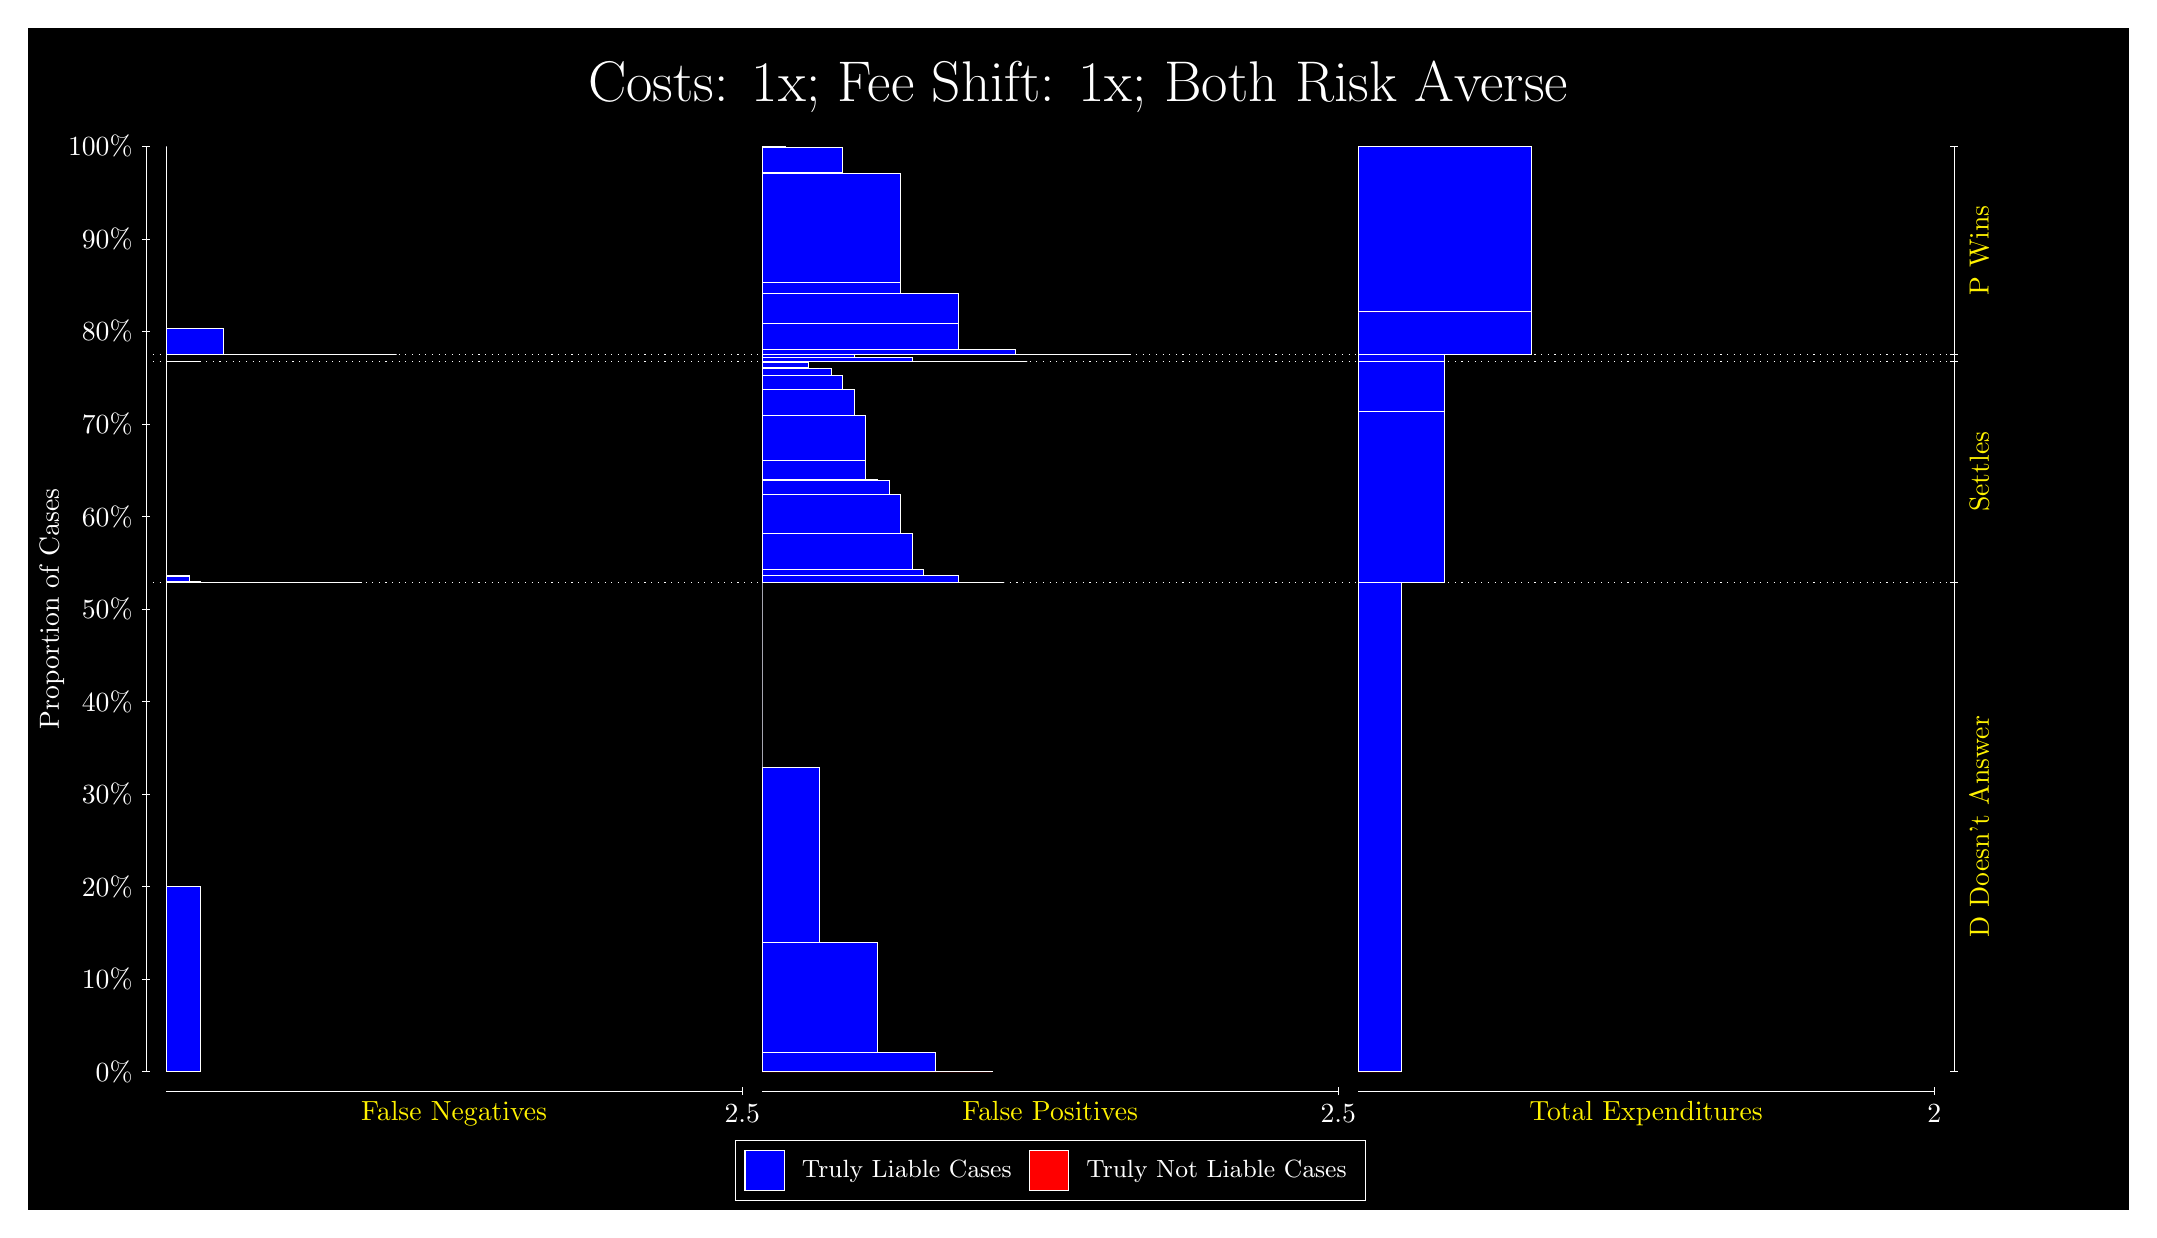
\begin{tikzpicture}
\draw[fill=black] (0,0) rectangle (26.667,15);
\draw[text=white] (0,13.5) rectangle (26.667,15) node[midway] {\huge Costs: 1x; Fee Shift: 1x; Both Risk Averse};
\draw[white, very thin] (1.5,1.75) -- (1.5,13.5);
\node[rotate=90, text=white, anchor=center] at (0.3, 7.625) {Proportion of Cases};
\draw[white, very thin] (1.45,1.75) -- (1.55,1.75);
\node[text=white, anchor=east] at (1.45, 1.75) {0\%};
\draw[white, very thin] (1.45,2.925) -- (1.55,2.925);
\node[text=white, anchor=east] at (1.45, 2.925) {10\%};
\draw[white, very thin] (1.45,4.1) -- (1.55,4.1);
\node[text=white, anchor=east] at (1.45, 4.1) {20\%};
\draw[white, very thin] (1.45,5.275) -- (1.55,5.275);
\node[text=white, anchor=east] at (1.45, 5.275) {30\%};
\draw[white, very thin] (1.45,6.45) -- (1.55,6.45);
\node[text=white, anchor=east] at (1.45, 6.45) {40\%};
\draw[white, very thin] (1.45,7.625) -- (1.55,7.625);
\node[text=white, anchor=east] at (1.45, 7.625) {50\%};
\draw[white, very thin] (1.45,8.8) -- (1.55,8.8);
\node[text=white, anchor=east] at (1.45, 8.8) {60\%};
\draw[white, very thin] (1.45,9.975) -- (1.55,9.975);
\node[text=white, anchor=east] at (1.45, 9.975) {70\%};
\draw[white, very thin] (1.45,11.15) -- (1.55,11.15);
\node[text=white, anchor=east] at (1.45, 11.15) {80\%};
\draw[white, very thin] (1.45,12.325) -- (1.55,12.325);
\node[text=white, anchor=east] at (1.45, 12.325) {90\%};
\draw[white, very thin] (1.45,13.5) -- (1.55,13.5);
\node[text=white, anchor=east] at (1.45, 13.5) {100\%};

\draw[white, very thin] (24.457,1.75) -- (24.457,13.5);
\draw[white, very thin] (24.407,1.75) -- (24.507,1.75);
\node[anchor=west] at (24.407, 1.75) {};
\draw[white, very thin] (24.407,7.9609) -- (24.507,7.9609);
\node[anchor=west] at (24.407, 7.9609) {};
\draw[white, very thin] (24.407,10.772) -- (24.507,10.772);
\node[anchor=west] at (24.407, 10.772) {};
\draw[white, very thin] (24.407,10.857) -- (24.507,10.857);
\node[anchor=west] at (24.407, 10.857) {};
\draw[white, very thin] (24.407,13.5) -- (24.507,13.5);
\node[anchor=west] at (24.407, 13.5) {};

\draw[white, very thin, fill=blue] (1.75,1.75) rectangle (2.1891,4.0986);
\draw[white, very thin, fill=red] (1.75,4.0986) rectangle (1.75,4.0986);
\draw[white, very thin, fill=blue] (1.75,4.0986) rectangle (1.75,7.9609);
\draw[white, very thin, fill=blue] (1.75,7.9609) rectangle (4.2384,7.9609);
\draw[white, very thin, fill=blue] (1.75,7.9609) rectangle (3.6529,7.9609);
\draw[white, very thin, fill=blue] (1.75,7.9609) rectangle (3.5065,7.9609);
\draw[white, very thin, fill=blue] (1.75,7.9609) rectangle (3.3602,7.9609);
\draw[white, very thin, fill=blue] (1.75,7.9609) rectangle (3.0674,7.9609);
\draw[white, very thin, fill=blue] (1.75,7.9609) rectangle (2.921,7.9609);
\draw[white, very thin, fill=blue] (1.75,7.9609) rectangle (2.7746,7.961);
\draw[white, very thin, fill=blue] (1.75,7.961) rectangle (2.6283,7.961);
\draw[white, very thin, fill=blue] (1.75,7.961) rectangle (2.4819,7.962);
\draw[white, very thin, fill=blue] (1.75,7.962) rectangle (2.3355,7.966);
\draw[white, very thin, fill=blue] (1.75,7.966) rectangle (2.1891,7.9799);
\draw[white, very thin, fill=blue] (1.75,7.9799) rectangle (2.0428,8.0415);
\draw[white, very thin, fill=blue] (1.75,8.0415) rectangle (2.0428,8.0514);
\draw[white, very thin, fill=blue] (1.75,8.0514) rectangle (1.8964,8.0517);
\draw[white, very thin, fill=red] (1.75,8.0517) rectangle (1.75,8.0517);
\draw[white, very thin, fill=blue] (1.75,8.0517) rectangle (1.75,10.772);
\draw[white, very thin, fill=blue] (1.75,10.772) rectangle (2.1891,10.773);
\draw[white, very thin, fill=red] (1.75,10.773) rectangle (1.75,10.773);
\draw[white, very thin, fill=blue] (1.75,10.773) rectangle (1.75,10.857);
\draw[white, very thin, fill=blue] (1.75,10.857) rectangle (4.6775,10.857);
\draw[white, very thin, fill=blue] (1.75,10.857) rectangle (3.9457,10.857);
\draw[white, very thin, fill=blue] (1.75,10.857) rectangle (3.2138,10.864);
\draw[white, very thin, fill=blue] (1.75,10.864) rectangle (2.4819,11.193);
\draw[white, very thin, fill=red] (1.75,11.193) rectangle (1.75,11.193);
\draw[white, very thin, fill=blue] (1.75,11.193) rectangle (1.75,13.5);
\draw[white, very thin, fill=red] (9.3189,1.75) rectangle (12.246,1.75);
\draw[white, very thin, fill=blue] (9.3189,1.75) rectangle (12.246,1.7524);
\draw[white, very thin, fill=blue] (9.3189,1.7524) rectangle (11.515,1.9936);
\draw[white, very thin, fill=blue] (9.3189,1.9936) rectangle (10.783,3.3977);
\draw[white, very thin, fill=blue] (9.3189,3.3977) rectangle (10.051,5.6124);
\draw[white, very thin, fill=blue] (9.3189,5.6124) rectangle (9.3189,7.9609);
\draw[white, very thin, fill=red] (9.3189,7.9609) rectangle (12.393,7.9609);
\draw[white, very thin, fill=blue] (9.3189,7.9609) rectangle (12.393,7.9609);
\draw[white, very thin, fill=red] (9.3189,7.9609) rectangle (12.1,7.9609);
\draw[white, very thin, fill=blue] (9.3189,7.9609) rectangle (12.1,7.9615);
\draw[white, very thin, fill=red] (9.3189,7.9615) rectangle (11.807,7.9615);
\draw[white, very thin, fill=blue] (9.3189,7.9615) rectangle (11.807,8.0487);
\draw[white, very thin, fill=blue] (9.3189,8.0487) rectangle (11.661,8.0545);
\draw[white, very thin, fill=red] (9.3189,8.0545) rectangle (11.515,8.0545);
\draw[white, very thin, fill=blue] (9.3189,8.0545) rectangle (11.515,8.0548);
\draw[white, very thin, fill=blue] (9.3189,8.0548) rectangle (11.368,8.1332);
\draw[white, very thin, fill=red] (9.3189,8.1332) rectangle (11.222,8.1332);
\draw[white, very thin, fill=blue] (9.3189,8.1332) rectangle (11.222,8.5832);
\draw[white, very thin, fill=blue] (9.3189,8.5832) rectangle (11.075,9.0869);
\draw[white, very thin, fill=blue] (9.3189,9.0869) rectangle (10.929,9.2596);
\draw[white, very thin, fill=blue] (9.3189,9.2596) rectangle (10.783,9.2666);
\draw[white, very thin, fill=blue] (9.3189,9.2666) rectangle (10.636,9.513);
\draw[white, very thin, fill=red] (9.3189,9.513) rectangle (10.636,9.513);
\draw[white, very thin, fill=blue] (9.3189,9.513) rectangle (10.636,10.088);
\draw[white, very thin, fill=blue] (9.3189,10.088) rectangle (10.49,10.415);
\draw[white, very thin, fill=blue] (9.3189,10.415) rectangle (10.344,10.593);
\draw[white, very thin, fill=blue] (9.3189,10.593) rectangle (10.197,10.682);
\draw[white, very thin, fill=blue] (9.3189,10.682) rectangle (10.051,10.682);
\draw[white, very thin, fill=blue] (9.3189,10.682) rectangle (9.9044,10.692);
\draw[white, very thin, fill=blue] (9.3189,10.692) rectangle (9.9044,10.753);
\draw[white, very thin, fill=blue] (9.3189,10.753) rectangle (9.758,10.767);
\draw[white, very thin, fill=blue] (9.3189,10.767) rectangle (9.6116,10.771);
\draw[white, very thin, fill=blue] (9.3189,10.771) rectangle (9.4652,10.772);
\draw[white, very thin, fill=blue] (9.3189,10.772) rectangle (9.3189,10.772);
\draw[white, very thin, fill=red] (9.3189,10.772) rectangle (12.686,10.772);
\draw[white, very thin, fill=blue] (9.3189,10.772) rectangle (12.686,10.772);
\draw[white, very thin, fill=blue] (9.3189,10.772) rectangle (11.954,10.774);
\draw[white, very thin, fill=blue] (9.3189,10.774) rectangle (11.222,10.827);
\draw[white, very thin, fill=blue] (9.3189,10.827) rectangle (10.49,10.857);
\draw[white, very thin, fill=blue] (9.3189,10.857) rectangle (9.758,10.857);
\draw[white, very thin, fill=red] (9.3189,10.857) rectangle (14.003,10.857);
\draw[white, very thin, fill=blue] (9.3189,10.857) rectangle (14.003,10.857);
\draw[white, very thin, fill=red] (9.3189,10.857) rectangle (13.271,10.857);
\draw[white, very thin, fill=blue] (9.3189,10.857) rectangle (13.271,10.859);
\draw[white, very thin, fill=red] (9.3189,10.859) rectangle (12.539,10.859);
\draw[white, very thin, fill=blue] (9.3189,10.859) rectangle (12.539,10.927);
\draw[white, very thin, fill=blue] (9.3189,10.927) rectangle (11.807,11.257);
\draw[white, very thin, fill=red] (9.3189,11.257) rectangle (11.807,11.257);
\draw[white, very thin, fill=blue] (9.3189,11.257) rectangle (11.807,11.636);
\draw[white, very thin, fill=blue] (9.3189,11.636) rectangle (11.075,11.777);
\draw[white, very thin, fill=red] (9.3189,11.777) rectangle (11.075,11.777);
\draw[white, very thin, fill=blue] (9.3189,11.777) rectangle (11.075,13.164);
\draw[white, very thin, fill=blue] (9.3189,13.164) rectangle (10.344,13.165);
\draw[white, very thin, fill=blue] (9.3189,13.165) rectangle (10.344,13.494);
\draw[white, very thin, fill=blue] (9.3189,13.494) rectangle (9.6116,13.494);
\draw[white, very thin, fill=blue] (9.3189,13.494) rectangle (9.6116,13.5);
\draw[white, very thin, fill=blue] (9.3189,13.5) rectangle (9.3189,13.5);
\draw[white, very thin, fill=red] (16.888,1.75) rectangle (17.437,1.75);
\draw[white, very thin, fill=blue] (16.888,1.75) rectangle (17.437,7.9609);
\draw[white, very thin, fill=red] (16.888,7.9609) rectangle (17.986,7.9609);
\draw[white, very thin, fill=blue] (16.888,7.9609) rectangle (17.986,10.135);
\draw[white, very thin, fill=red] (16.888,10.135) rectangle (17.986,10.135);
\draw[white, very thin, fill=blue] (16.888,10.135) rectangle (17.986,10.772);
\draw[white, very thin, fill=red] (16.888,10.772) rectangle (17.986,10.772);
\draw[white, very thin, fill=blue] (16.888,10.772) rectangle (17.986,10.857);
\draw[white, very thin, fill=red] (16.888,10.857) rectangle (19.083,10.857);
\draw[white, very thin, fill=blue] (16.888,10.857) rectangle (19.083,11.399);
\draw[white, very thin, fill=red] (16.888,11.399) rectangle (19.083,11.399);
\draw[white, very thin, fill=blue] (16.888,11.399) rectangle (19.083,13.5);
\draw[white, dotted] (1.5,7.9609) -- (24.457,7.9609);
\draw[white, dotted] (1.5,10.772) -- (24.457,10.772);
\draw[white, dotted] (1.5,10.857) -- (24.457,10.857);
\draw[white, very thin] (1.75,1.5) -- (9.0689,1.5);
\node[text=yellow, anchor=north] at (5.4094, 1.5) {False Negatives};
\draw[white, very thin] (9.0689,1.45) -- (9.0689,1.55);
\node[text=white, anchor=north] at (9.0689, 1.45) {2.5};

\draw[white, very thin] (9.3189,1.5) -- (16.638,1.5);
\node[text=yellow, anchor=north] at (12.978, 1.5) {False Positives};
\draw[white, very thin] (16.638,1.45) -- (16.638,1.55);
\node[text=white, anchor=north] at (16.638, 1.45) {2.5};

\draw[white, very thin] (16.888,1.5) -- (24.207,1.5);
\node[text=yellow, anchor=north] at (20.547, 1.5) {Total Expenditures};
\draw[white, very thin] (24.207,1.45) -- (24.207,1.55);
\node[text=white, anchor=north] at (24.207, 1.45) {2};

\node[text=yellow, centered, rotate=90] at (24.777, 4.8555) {D Doesn't Answer};
\node[text=yellow, centered, rotate=90] at (24.777, 9.3666) {Settles};

\node[text=yellow, centered, rotate=90] at (24.777, 12.179) {P Wins};

\draw (12.978300999999998,1.5) node[draw=none] (baseCoordinate) {};
\begin{scope}[align=center]
        \matrix[scale=0.5, draw=white, below=0.5cm of baseCoordinate, nodes={draw}, column sep=0.1cm]{
            \node[rectangle, draw, minimum width=0.5cm, minimum height=0.5cm, fill=blue] {}; &
            \node[draw=none, font=\small, text=white] (B) {Truly Liable Cases}; &
            \node[rectangle, draw, minimum width=0.5cm, minimum height=0.5cm, fill=red] {}; &
            \node[draw=none, font=\small, text=white] (B) {Truly Not Liable Cases}; \\
            };
\end{scope}

\end{tikzpicture}
\end{document}